\documentclass[../catalog.tex]{subfiles}

\begin{document}

Within an attribute-oriented data model, relational joins cannot be
treated as scary, exceptional operations, but must rather be viewed as
commonplace, everyday tools. Even the most basic aggregation of data —
obtaining a consistent view of domain entities over time — requires
joining potentially many attributes. Robustly maintaining high-arity
joins for many concurrent users with low-latency and high-throughput
is therefore the defining problem of the 3DF architecture.

Join operators must maintain state to buffer inputs on either side,
until matching inputs from the other side arrive (and vice versa) or
the epoch closes. Systems like Kafka Streams enforce sliding,
fixed-size window semantics (\cite{kafkadocs}) to put a bound on the
state maintained by each join operator. Differential Dataflow
maintains such state in arrangements (c.f. chapter
\ref{background-differential}) that are compacted as the computation
makes progress (i.e. epochs are completed). Differential's
\texttt{join} operator will therefore arrange both of its input
collections on the join variables, should they not already be
available in arranged form.

For higher-arity joins this becomes problematic, because the output of
the first two-way join will be fed as an input into the second two-way
join, and so on. At each stage along the spine (except for the very
last), intermediate join results will therefore be maintained in
arranged form. This is illustrated in
\autoref{fig:join-at-a-time-plan}.

\begin{figure}[h!]
  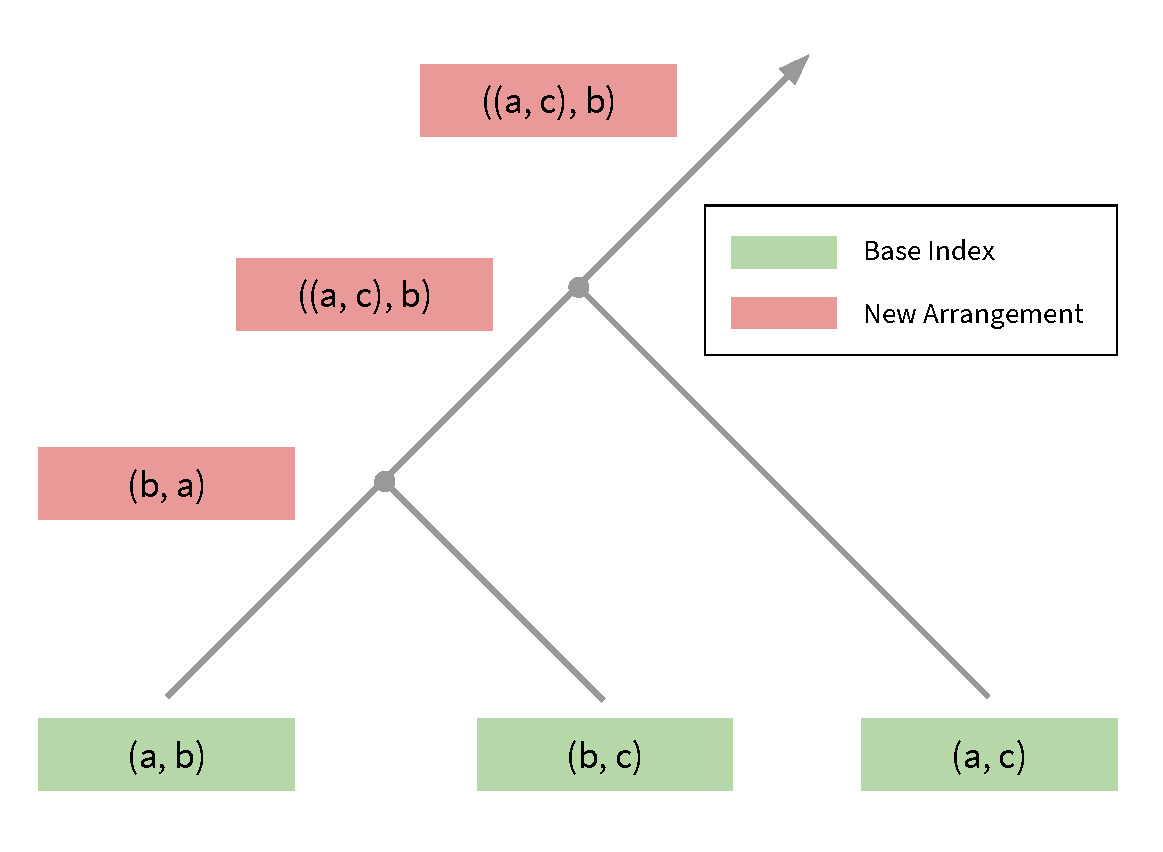
\includegraphics[width=1.0\linewidth]{diagrams/join-at-a-time}
  \caption{Join At A Time}
  \label{fig:join-at-a-time-plan}

  \medskip
  \small

  An exemplary three-way joiin implemented via a join-at-a-time
  plan. Base relations are in green and are shared across all
  queries. Arrangements in red hold intermediate join state, are
  created on-the-fly, and not shared with other dataflows.
\end{figure}

Depending on the selectivity of the various join stages, this can lead
to significant space overheads. Worse, in our continuous query
processing setting, erroneously estimating intermediate cardinalities
will therefore cause disastrous complexity in both time \emph{and}
space.

\subsection{Example}

Intermediate join state becomes especially apparent in star-joins
along highly correlated columns, e.g. one-to-one relations with very
similar cardinalities and low selectivity. Unfortunately this is a
very common use case in our attribute-oriented data model. Consider
the following query.

\begin{verbatim}
[:find ?person
 :where
 [?person :person/firstname _]
 [?person :person/lastname _]
 [?person :person/gender _]
 [?person :person/birthday _]
 [?person :person/creation-date _]
 [?person :person/ip _]
 [?person :person/browser _]]
\end{verbatim}

This query requires a seven-way join on all person ids, aggregating
seven different person attributes back into a consistent view of each
person. Within the LDBC dataset (\cite{erling2015ldbc}) for example,
every person carries all seven of these attributes. Therefore all
relations are of the same size and map one-to-one from person ids to
the associated values. Because of this, implementing this query as six
consecutive two-way joins leads to a five-fold increase in the number
of tuples maintained by this dataflow \emph{regardless of the chosen
  join order}.

We encounter an even more pronounced version of this problem on cyclic
sub-graph queries, such as the triangle search:

\begin{verbatim}
[:find ?a ?b ?c
 :where
 [?a :person/knows ?b]
 [?b :person/knows ?c]
 [?a :person/knows ?c]]
\end{verbatim}

Here the attributes do not have a one-to-one correspondence anymore (a
few celebrities might have in-degrees in the millions, whereas most
people are in mutual friendship with a few hundred others) and
intermediate result sets can grow super-linearly.

\subsection{Remedy}

Adapting the incremental join view techniques from
\cite{blakeley1986efficiently}, we can break up our queries along
their potential sources of change
(c.f. \autoref{fig:delta-query-plan}). In our example, any of the
comment attributes may change arbitrarily, which means we will end up
with six separate queries.

\begin{figure}[h!]
  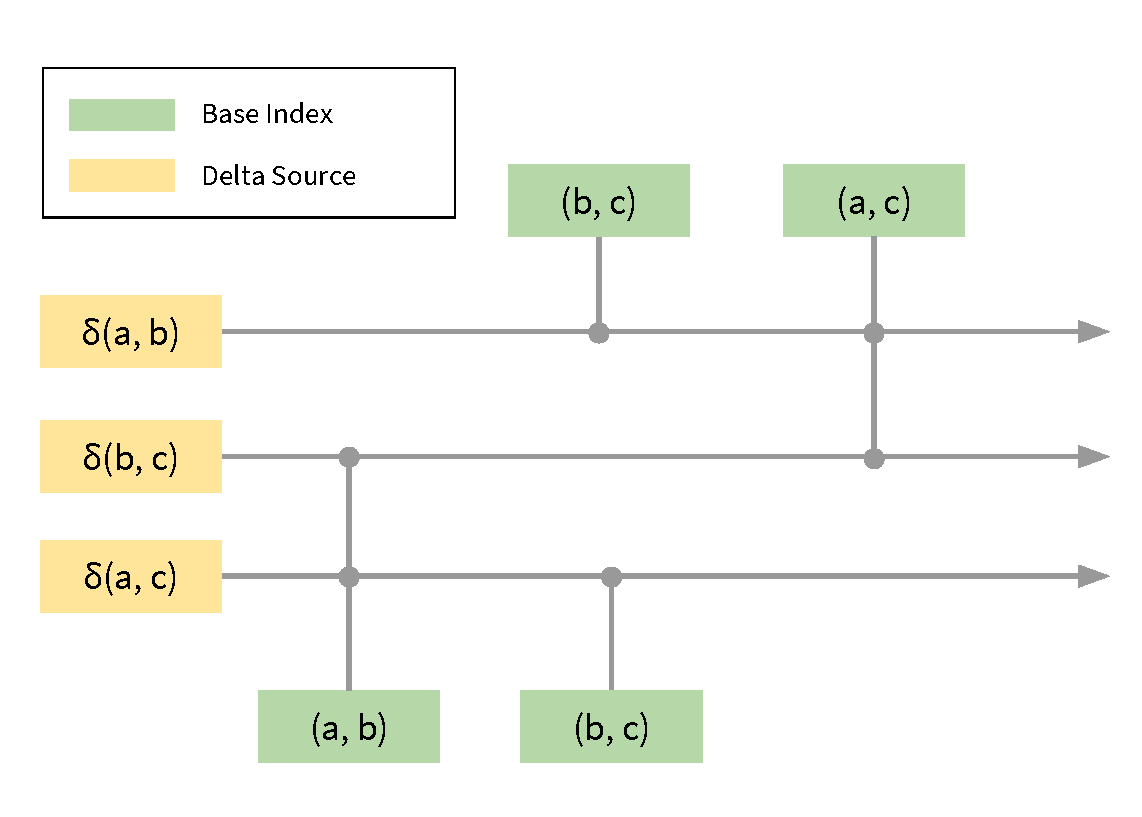
\includegraphics[width=1.0\linewidth]{diagrams/delta-queries}
  \caption{Delta Queries}
  \label{fig:delta-query-plan}

  \medskip
  \small
  
  An exemplary three-way join implemented via delta-queries. Three
  independent dataflows are required, each handling changes to a
  specific base relation. These delta sources are stateless.
\end{figure}

What is different about the resulting plans, is that, given an indexed
representation of all attributes, they can be implemented in an
otherwise stateless manner. They do not need to maintain intermediate
arrangements as was the case for the traditional join operator. This
allows us to decouple the memory use of our join processing from the
number of active queries and the complexity of the joins, and instead
bound it in the number and size of attributes maintained. There is a
trade-off of course, as transforming plans into delta queries leads to
an increase in the number of dataflow elements.

Within any given delta flow, an attribute may only appear at a
position where either of its sides is already bound by the tuples
flowing through it, in order to avoid having to produce the entire
relation for each incoming tuple. We therefore would want to keep
attributes indexed in both directions (from entity id to value and the
other way around), to increase the number of possible plans available
to us.

Another subtle issue, identified in \cite{dogsdogsdogs}, arises when
implementing delta queries within the dataflow model. Simultaneous
updates to multiple of the participating attributes can lead to
redundant derivations of the same result tuple. We must be careful to
impose a logical order on the execution. This implementation detail is
described later in \autoref{impl-altneu}.

\subsection{Evaluation}

We show that joins of arbitrary arity implemented with delta queries
maintain no intermediate tuples, whereas the same joins implemented as
join-at-a-time plans store intermediate tuples in proportion to the
size of the base relations and the arity of the join. Both approaches
require base relations in arranged form, which are shared across all
queries. We find that delta queries do not adversely affect update
latencies in a significant way.

Using the LDBC data generators we generated a dataset simulating the
social network activity of ~10,000 persons. On this we ran subsets of
the above conjunctive query on attributes of persons, increasing the
number of clauses participating in the join with each run. These runs
were performed with the dataset fully loaded into 3DF and without
streaming updates.

During each run we measured the number of tuples maintained across
arrangements within the query dataflow. Differential provides event
streams containing information about the logical size of
arrangements. From those events, the number of tuples within an
arrangement is easily inferred. Implementation details of the logging
instrumentation are covered in \autoref{logging}.

\begin{figure}[h!]
  \begin{subfigure}{.5\textwidth}
    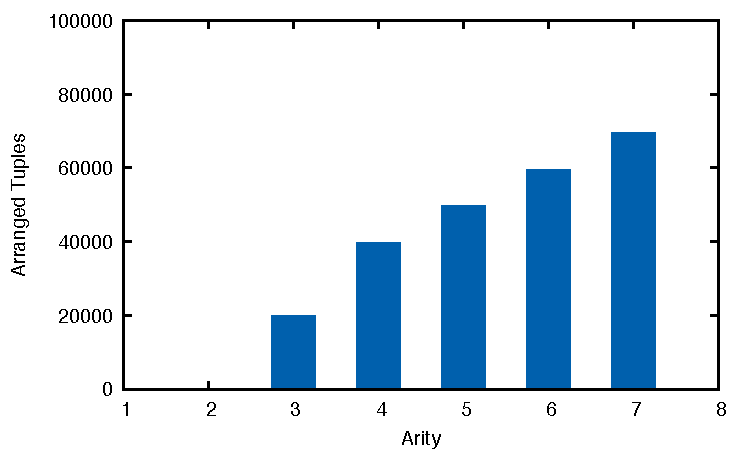
\includegraphics[width=1.0\linewidth]{results/join-state/out/tuples_join}
    \caption{Join-at-a-Time}
  \end{subfigure}
  \begin{subfigure}{.5\textwidth}
    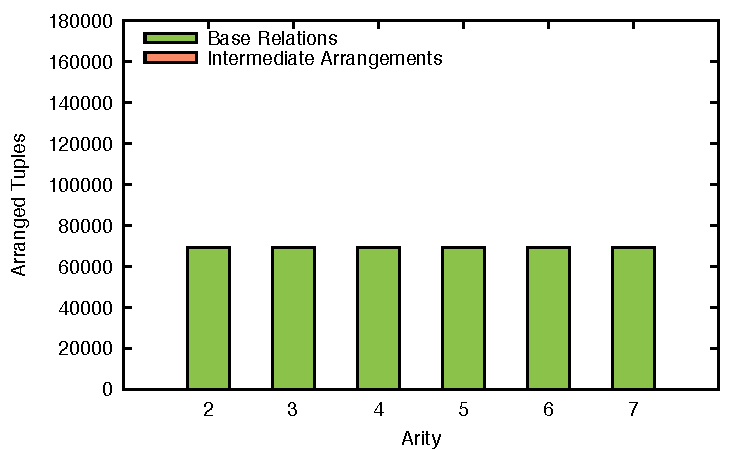
\includegraphics[width=1.0\linewidth]{results/join-state/out/tuples_delta}
    \caption{Delta Queries}
  \end{subfigure}

  \caption{Total Number of Tuples in Arrangements}
  \label{fig:tuple-counts}
  \medskip
  \small

  Total number of tuples maintained across base relations and
  intermediate join state, measured on join-at-a-time plans (a) and
  delta query plans (b) of increasing arity. Tuples in intermediate
  arrangements are not shared between queries. Intermediate state
  grows proportional to join arity for join-at-a-time plans, whereas
  no intermediate state is required for delta queries.
\end{figure}

\autoref{fig:tuple-counts} shows the total number of tuples held in
arrangements, after each join produced a complete initial result
set. Tuple counts are broken down into those held in base relations,
which are shared across all queries, and those stored in intermediate
arrangements created by the join operator. We observe that for
join-at-a-time plans, the number of arranged intermediate tuples grows
linearly with the arity of the join, whereas no intermediate tuples
are stored when using delta queries on joins of arbitrary arity. Note
that our join-at-a-time implementation does not yet make full use of
all available base relations for higher arities. An optimal
implementation should be expected to produce around half the absolute
number of intermediate tuples.

Arguably join-at-a-time plans allow for a lower overall memory
footprint if the number of queries is low and join arities are small
in comparison to the number and size of base relations, because
reverse indices on base relations wouldn't have to be
maintained. However these assumptions do not hold for our setting.

\begin{figure}[h!]
  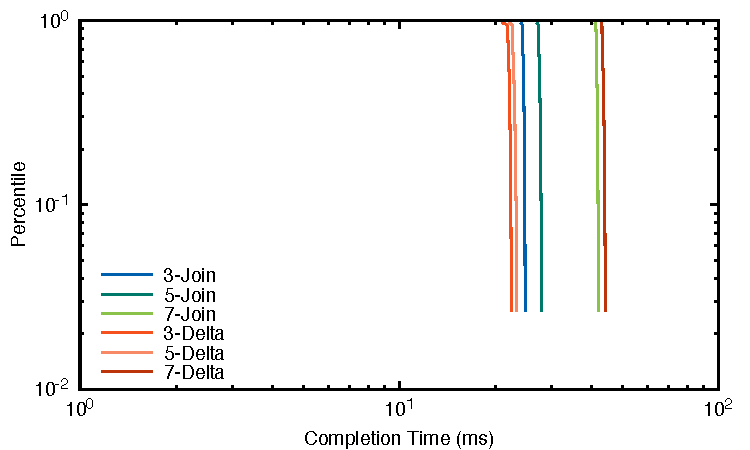
\includegraphics[width=1.0\linewidth]{results/join-state/out/all_cdfs}
  \caption{Latency CCDFS}
  \label{fig:arity-latencies}
  \medskip
  \small

  Complementary CDFs of join completion times for each round of
  inputs, when streaming inputs into pre-registered joins of
  increasing arity. Delta queries do not adversely effect update
  latencies.
\end{figure}

We then inverted the setup, first creating join dataflows before
streaming in all person attributes from the LDBC dataset. We measured
completion times for each distinct batch of inputs. The resulting
distributions are shown in \autoref{fig:arity-latencies}. We observe
that both join strategies produce very similar distributions with
increasing arity.

Delta queries thus allow us to trade dataflow size in return for a
predictable memory footprint, and to do so without affecting latencies
in a significant way. Considering only selections, projections, and
n-way joins, the overall system could be configured to use only memory
proportional to the number and size of the base relations. No
additional operator state is required, independent of the number of
queries and the arity of the joins within them.

Additionally, delta queries decouple space from time complexity. Using
traditional tree joins, a sub-optimal join plan incurs both a heavy
computational cost as well as space overheads, due to the sheer number
of intermediate tuples materialized and maintained in
arrangements. Delta queries still have to spend time processing large
numbers of tuples, but without the need to index them at intermediate
stages.

While we must at some point take measures to keep the overall size of
the dataflow manageable (as will be the topic of
\autoref{case-redundant-dataflows}), we conclude that delta queries
are a powerful technique in many common scenarios.

\end{document}
